% Chapter 2
\chapter{Background}
\label{ch:background}

This chapter explains the parts that Lizard combines. It uses one notation for all formulas. A sequence has the positions $1, \dots, L$. At position $i$, an attention head has the query $\vq_i$, and each position $t$ has a key $\vk_t$ and a value $\vv_t$. The head dimension is $d$.

\section{The transformer and causal softmax attention}
\label{sec:softmax}

A decoder-only transformer~\cite{vaswani2017} has a stack of layers. Each layer has an attention block and an MLP block. The attention block projects its input $\vx_i$ into queries, keys and values with the matrices $W_Q$, $W_K$ and $W_V$. Then each head computes a weighted mean of the earlier values:
\begin{equation}
\vy_i = \sum_{t=1}^{i} \frac{\exp\!\left(\vq_i^\top \vk_t / \sqrt{d}\right)}{\sum_{j=1}^{i} \exp\!\left(\vq_i^\top \vk_j / \sqrt{d}\right)}\, \vv_t .
\label{eq:softmax}
\end{equation}
The sum stops at $i$, so a token sees only earlier tokens. This is the \emph{causal} mask. The output projection $W_O$ then mixes the heads. The weights of a row are positive and sum to 1. Thus each output is a weighted mean of values. The weights can be sharp. For example, a head can put almost all weight on the previous token.

The teacher of this thesis is Llama-3.2-1B~\cite{llama3}. It has 16 layers, a hidden size of 2048 and 32 attention heads with a head dimension of 64. The keys and the values use 8 heads, and groups of query heads share them.

\section{Rotary position embedding}
\label{sec:rope}

\Cref{eq:softmax} has no information about the positions. A transformer must add this information. Llama uses the rotary position embedding (RoPE)~\cite{roformer}. RoPE splits each query and each key into pairs of numbers. It rotates each pair by an angle that grows with the position $i$. Each pair has its own speed of rotation. Let $R_i$ be the rotation for position $i$. Then the score becomes
\begin{equation}
\left(R_i \vq_i\right)^\top \left(R_t \vk_t\right) = \vq_i^\top R_{t-i}\, \vk_t .
\label{eq:rope}
\end{equation}
The rotation matrices are orthogonal, so the score depends only on the distance $t - i$ and not on the absolute positions. Llama-3.2-1B uses the base frequency 500,000. RoPE needs no extra memory. A key gets its rotation one time, at its own position, and the cache keeps the rotated key.

RoPE is important for this thesis. With RoPE, a head can find \enquote{the token one position back} from the positions alone. Without RoPE, a head sees only the content of the tokens.

\section{The cost of softmax attention}
\label{sec:cost}

For a sequence of length $L$, \cref{eq:softmax} computes $L^2/2$ scores in each head. Thus the time grows with $L^2$. During generation, each new token needs the keys and values of all earlier tokens. Thus the cache grows with $L$, and the time for each new token also grows with $L$. \Cref{sec:intro-cost} gives the size of the cache for the teacher.

\section{Linear attention and feature maps}
\label{sec:linear}

Linear attention~\cite{katharopoulos2020} replaces $\exp(\vq^\top\vk/\sqrt{d})$ with a product $\phi(\vq)^\top \phi(\vk)$ of a feature map $\phi$. The feature map gives positive values. Then the output is
\begin{equation}
\vy_i = \frac{\phi(\vq_i)^\top \sum_{t=1}^{i} \phi(\vk_t)\, \vv_t^\top}{\phi(\vq_i)^\top \sum_{j=1}^{i} \phi(\vk_j)} .
\label{eq:linear}
\end{equation}
The two sums do not depend on the query. Thus the model can keep them as a state and add one term for each new token:
\begin{equation}
\vS_i = \vS_{i-1} + \phi(\vk_i)\, \vv_i^\top, \qquad \vz_i = \vz_{i-1} + \phi(\vk_i), \qquad \vy_i = \frac{\phi(\vq_i)^\top \vS_i}{\phi(\vq_i)^\top \vz_i} .
\label{eq:linear-recurrent}
\end{equation}
The state $\vS_i$ has the size $f \times d$, with $f$ features. It does not grow with the length. The time for each new token is constant. The price is accuracy: a fixed state cannot store every detail of a long text.

\section{Hedgehog feature maps}
\label{sec:hedgehog}

The choice of $\phi$ decides how well \cref{eq:linear} can copy softmax attention. Hedgehog~\cite{hedgehog} learns the feature map. It uses a matrix $W$ and two exponentials:
\begin{equation}
\phi(\vx) = \left[\, \mathrm{softmax}(\vx W) \oplus \mathrm{softmax}(-\vx W) \,\right] .
\label{eq:hedgehog}
\end{equation}
Here $\oplus$ joins two vectors. With $W \in \R^{d \times f}$, each query and each key gets $2f$ features. All features are positive. The paper of Lizard gives the form with $\exp$ in its Section~4, but its Table~13 gives the softmax form. The code of this work uses the softmax form. Hedgehog trains $W$ so that the weights of linear attention look like the weights of softmax attention: positive, monotonic in the score, and sometimes sharp.

\section{Gated linear attention}
\label{sec:gla}

Plain linear attention gives the same weight to old tokens and new tokens. Gated linear attention (GLA)~\cite{gla} adds a gate $\gamma_l \in (0, 1)$ at each position. The gate makes old tokens less important. In the form of Lizard, with one scalar gate for each position, the output is
\begin{equation}
\vy_i = \frac{\phi_q(\vq_i)^\top \sum_{t=1}^{i} \left( \prod_{l=t+1}^{i} \gamma_l \right) \phi_k(\vk_t)\, \vv_t^\top}
{\phi_q(\vq_i)^\top \sum_{j=1}^{i} \left( \prod_{l=j+1}^{i} \gamma_l \right) \phi_k(\vk_j)} .
\label{eq:gla}
\end{equation}
The recurrent form multiplies the state by the gate before it adds the new token: $\vS_i = \gamma_i \vS_{i-1} + \phi_k(\vk_i)\vv_i^\top$. The two forms give the same output (\cref{app:formulas}). The product of the gates is the weight that a token keeps after some steps. With $\gamma = 0.99$, a token keeps 28\% of its weight after 128 steps. With $\gamma = 0.999$, it keeps 88\%. The gate is the only source of position information in this branch. It prefers recent tokens, but it cannot select one exact position.

\section{Sliding window attention and attention sinks}
\label{sec:swa}

Sliding window attention computes \cref{eq:softmax} over the last $w$ tokens only. Its cost for each token does not grow with the length, and it is exact inside the window. It cannot see tokens before the window.

Softmax models often put a large weight on the first token of a sequence, even when this token has no meaning for the task. Xiao et al.~\cite{streamingllm} call this token an \emph{attention sink}. A window that removes the first token loses this place for extra weight, and the model gets worse. Lizard adds $m$ learnable sink logits $t_1, \dots, t_m$ to the denominator of the window:
\begin{equation}
\hat\vy^{\text{win}}_i = \frac{\sum_{t=i-w+1}^{i} \exp\!\left(\vq_i^\top \vk_t/\sqrt{d}\right) \vv_t}{\sum_{j=1}^{m} \exp(t_j) + \sum_{t=i-w+1}^{i} \exp\!\left(\vq_i^\top \vk_t/\sqrt{d}\right)} .
\label{eq:window}
\end{equation}
The sinks take part of the weight but add no value. Thus the window weights sum to a number $\rho_i \le 1$. \Cref{fig:patterns} shows which keys each type of attention uses.

\begin{figure}[t]
\centering
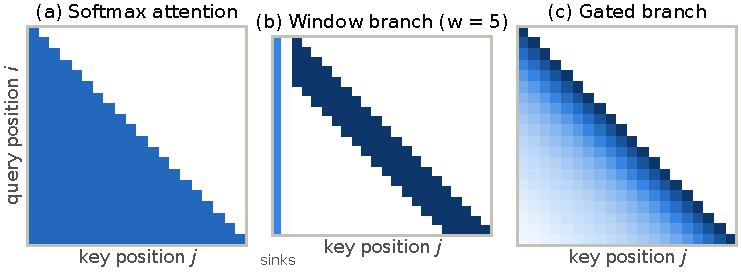
\includegraphics[width=\linewidth]{attention_patterns}
\caption[Keys that each type of attention uses]{Keys that each type of attention uses, in a toy example with 20 positions. Each row is a query and each column is a key. Darker cells have more weight. (a)~Softmax attention can use every earlier key. (b)~The window branch uses only the last $w$ keys, plus the sink logits on the left. (c)~The gated branch uses every earlier key, but the gate makes the weight smaller with the distance. Panel (c) uses a constant gate of 0.82.}
\label{fig:patterns}
\end{figure}

\section{Knowledge distillation and attention transfer}
\label{sec:distill}

In knowledge distillation~\cite{hinton2015}, a student model learns from the outputs of a teacher model. Linearization uses a special form: the student and the teacher have the same weights, except for the attention. Thus each student attention layer can learn directly from the teacher attention layer. The loss compares the two outputs of each layer with the mean squared error (MSE). This is \emph{attention transfer}. Each student layer gets the input of the teacher layer, not the output of the student layer before it. Thus an error in one layer does not change the input of the next layer during this training.

\section{Low-rank adaptation}
\label{sec:lora}

Attention transfer trains each layer alone. The full model can still lose quality. A second stage trains the whole model with the next-token loss. LoRA~\cite{lora} makes this stage cheap. It keeps a weight matrix $W$ frozen and adds a product of two small matrices: $W + \frac{\alpha_{\text{LoRA}}}{r} BA$, with the rank $r$. In this work, $r = 8$ and $\alpha_{\text{LoRA}} = 16$. With LoRA on the four attention projections, stage 2 trains 1,703,936 parameters, which is approximately 0.14\% of the model.

\section{How the harness scores multiple-choice tasks}
\label{sec:scoring}

The evaluation of this thesis does not let the model write an answer. For each question, the harness builds one text for each answer option. It computes the log-likelihood of the option after the question. The option with the highest value counts as the answer of the model. The metric \code{acc} uses the raw log-likelihood. The metric \code{acc_norm} divides it by the length of the option text, so that long options are not at a disadvantage.

MMLU uses a different format. The prompt lists four options with the letters A to D and ends with \enquote{Answer:}. The harness compares the log-likelihoods of the four tokens \enquote{ A} to \enquote{ D}. The model must therefore connect its knowledge with the right letter. PIQA and ARC use the full text of each option, so a preference for one letter has no effect there.

\section{The benchmarks}
\label{sec:benchmarks}

\Cref{tab:benchmarks} lists the benchmarks of this thesis. The paper of Lizard uses the same six benchmarks in its Table~9.

\begin{table}[ht]
\centering
\small
\caption[The benchmarks of this thesis]{The benchmarks of this thesis. All tasks are multiple choice. MMLU uses 5 examples before each question (5-shot). The other tasks use no examples (0-shot).}
\label{tab:benchmarks}
\begin{tabularx}{\linewidth}{@{}lLrcc@{}}
\toprule
Benchmark & Content & Questions & Options & Metric of the paper \\
\midrule
MMLU~\cite{mmlu} & Knowledge in 57 subjects, from high school to professional level & 14,042 & 4 & \code{acc}, 5-shot \\
PIQA~\cite{piqa} & Physical commonsense: a goal and two solutions & 1,838 & 2 & \code{acc} \\
ARC-Easy~\cite{arc} & Grade-school science questions, Easy set & 2,376 & 4 & \code{acc} \\
ARC-Challenge~\cite{arc} & Grade-school science questions, Challenge set & 1,172 & 4 & \code{acc_norm} \\
HellaSwag~\cite{hellaswag} & The most probable end of a short story & 10,042 & 4 & \code{acc_norm} \\
WinoGrande~\cite{winogrande} & Pronoun resolution in a sentence & 1,267 & 2 & \code{acc} \\
\bottomrule
\end{tabularx}
\end{table}

The chance level is 25\% for four options and 50\% for two options. The teacher is a small model, and it gets only 31.0 on MMLU in the paper. Thus the MMLU scores of all 1B models lie close to chance, and small differences need many questions. Appendix~\ref{app:definitions} gives short definitions of further terms, such as packing and padding.
